\indent Na etapie projektowania układu sterowania uchwytem wyodrębnione zostały podstawowe bloki funkcjonalne przedstawione na rys. \ref{schematpogladowy}. Obejmują one między innymi czujniki pomiarowe takie jak enkodery będące częścią istniejącej konstrukcji mechanicznej, sterowniki silników krokowych oraz główne urządzenie zarządzające.

\begin{figure}[!htb]
    \centering
    \resizebox{16cm}{!}{
    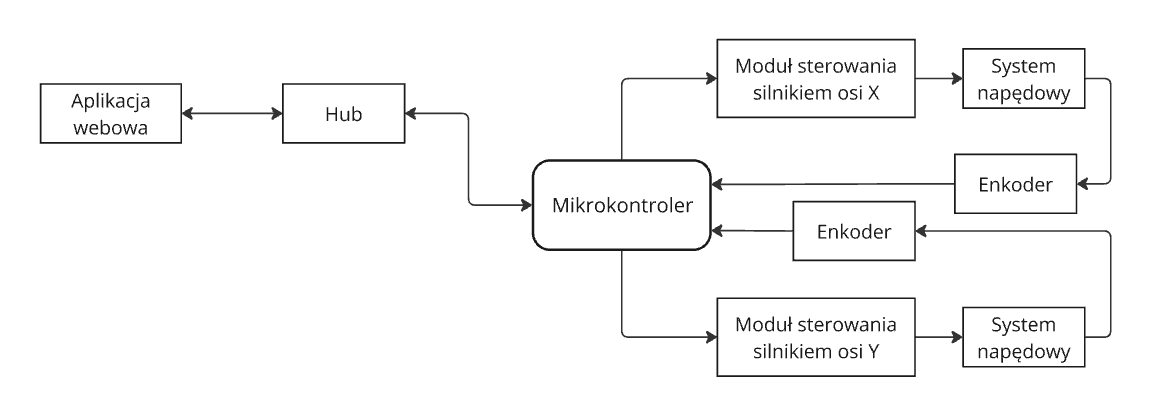
\includegraphics{testy/schematelementow.png}}
    \caption{Schemat elementów systemu}
     \label{schematpogladowy}
\end{figure}

\noindent Głównym elementem odpowiedzialnym za zarządzanie całym procesem jest mikrokontroler, pełniący rolę jednostki sterującej. Odbiera i przetwarza dane pochodzące z aplikacji webowej, w tym z warstwy frontendowej (interfejs użytkownika) oraz backendowej, którą w tym przypadku stanowi WebSocket. Ponadto odpowiada za komunikację zarówno z frontendem, jak i z serwerem działającym na STM32. Wymiana informacji między interfejsem użytkownika, a mikrokontrolerem STM32, odbywa się za pośrednictwem połączenia ethernetowego z protokołem TCP. Na STM32 działa serwer, który komunikuje się z urządzeniem sieciowym (hubem) i obsługuje przesył danych.

\noindent Po odebraniu i odpowiednim przetworzeniu danych z aplikacji webowej generowane są sygnały sterujące, które są przesyłane do modułów napędowych. Mikrokontroler wysyła kilka rodzajów sygnałów takich jak CLK (sygnał zegara), DIR (kierunek) oraz EN (zezwolenie na pracę), wpływając na działanie sterowników. Enkodery stanowiąc sprzężenie zwrotne za pośrednictwem interfejsu BISS-C, zwracają informacje do urządzenia sterującego, co pozwala na precyzyjne monitorowanie bieżącego stanu systemu. Silniki wraz z odpowiednią przekładnią tworząc system napędowy umożliwiają realizację zamierzonego ruchu, przekładając sygnały sterujące na odpowiednie obroty i moment obrotowy.

\noindent Mikrokontroler utrzymuje ruch platformy poprzez obliczanie zaimplementowanego algorytmu regulacji w celu ograniczenia uchybu kąta do przedziału wyznaczanego przez tzw. obszar tolerancji błędu (strefę nieczułości). Oznacza to, że system kontynuuje działanie, dopóki różnica między zadaną a rzeczywistą pozycją platformy przekracza określoną wartość progową. Taka konfiguracja pozwala na prostą realizację zadania sterowania przy ograniczeniu wrażliwości na błędy pomiarowe. Na etapie projektowania układu założono, że tak strategia powinna pozwolić uzyskać założony poziom dokładności. %płynne i stabilne %działanie całego układu, %zapewniając wysoką %dokładność oraz %skuteczność sterowania. 

%%%%%%%%%%%%%%%%%%%%%%%%%%%%%%%%%%% SILNIK %%%%%%%%%%%%%%%%%%%%%%%%%%%%%%%%%%%%%%

\section{Silniki}
Układ wykonawczy stanowi bardzo istotny element urządzenia pozycjonującego, dla którego opracowano układ sterowania. Konstrukcja  uchwytu oryginalnie została wyposażona w silniki krokowe, które choć nie zapewniają dużej dynamiki ruchu, to jednak umożliwiają precyzyjne sterowanie pozycyjne bez stosowania złożonego algorytmu pracującego w pętli zewnętrznej. Jest to uzyskiwane dzięki zasadzie działania tej grupy silników, które konstrukcyjnie zapewniają stabilne położenia wirnika

Z punktu widzenia działania układu istotne było dobranie odpowiedniej konfiguracji łączeniowej silników. Konfiguracje te obejmują: tryb unipolarny i tryb bipolarny w wersji szeregowej i równoległej - por. rys. \ref{fig:silnik}. 



%Z tego powodu przeanalizowano trzy sposoby podłączenia %\reviewdp{uzwojeń} silnika krokowego i wybrano \reviewdp{najlepszy}, dostosowany do warunków pracy. Wspomnijmy kilka słów na temat analizy wspomnianych wariantów.

\begin{figure}[!htb]
    \centering
    \resizebox{15cm}{!}{
    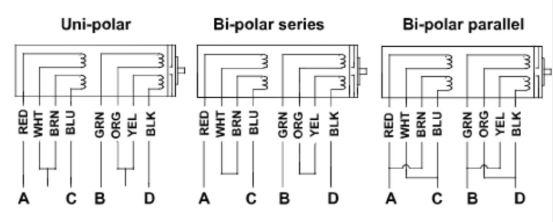
\includegraphics{pictures/silniki.png}}
    \caption{Sposoby podłączenia silników \cite{bipolarunipolar}}
    \label{fig:silnik}
\end{figure}

\begin{enumerate}
    \item \textbf{Połączenie unipolarne}\\
    Wyróżnia się z pewnością prostotą sterowania, a do jego prawidłowego działania wystarczy aktywować uzwojenia silnika w ustalonej kolejności. Zmiana kierunku obrotu wymaga jedynie odwrócenia sekwencji podawanego prądu. Pomimo swoich zalet jest ograniczone do generowania dużego momentu obrotowego. Z tego powodu nie stanowi odpowiedniego wyboru dla zastosowań wymagających większej siły np. obsługa dużej platformy.
    \item \textbf{Połączenie bipolarne szeregowe}\\
    W tym przypadku uzwojenia są połączone w taki sposób, że zwiększa się indukcyjność obwodu. Prowadzi to do ograniczenia stromości przepływu prądu przez uzwojenia, utrudniając pracę silnika przy wyższych częstotliwościach. Połączenie to generuje duży moment obrotowy, jednak ogranicza maksymalną prędkość obrotową. Jest ono odpowiednie dla aplikacji, gdzie wysoki moment jest priorytetem, a prędkość odgrywa mniejszą rolę.
    \vspace{1cm}
    \item \textbf{Połączenie bipolarne równoległe}\\
    Konfiguracja równoległa w połączeniu bipolarnym działa odwrotnie do połączenia szeregowego. Prąd dzieli się na dwa uzwojenia zmniejszając wpływ indukcyjności i pozwala na szybsze przełączanie faz w silniku. Dzięki temu silnik jest zdolny do pracy przy wyższych prędkościach, jednocześnie utrzymując relatywnie wysoki moment obrotowy. Spadek momentu wraz ze wzrostem prędkości nie jest tak gwałtowny jak w przypadku połączenia szeregowego czyniąc tę konfigurację bardziej uniwersalną dla szerokiego zakresu zastosowań.
\end{enumerate}

\vspace{1cm}

\noindent Warunki pracy rozważanego uchwytu wymagają użycia niewielkich prędkości obrotowych przy stosunkowo dużych wartościach momentu obrotowego \cite{silniki}. Z tego względu zdecydowano się na typ bipolarny szeregowy. \newline
\noindent Oprócz dobrania prawidłowej konfiguracji połączeń, praca silnika krokowego, a zwłaszcza precyzja pozycjonowania jego wirnika zależy od użytej strategii sterowania powiązanej z liczbą kroków w trakcie jednego obrotu. Można w tym obszarze wyróżnić pracę pełnokrokową (full step) lub pracę mikrokrokową (microstepping). Wariant \textbf{\textit{Full Step}} charakteryzuje się wykonywaniem pełnych kroków. Silnik wykorzystuje całkowity potencjał momentu obrotowego i z racji na mniej skomplikowane sterowanie pozwala uzyskać zwiększoną niezawodność. W przeciwieństwie do trybu pełnokrokowego działa \textbf{\textit{Mircostepping}} dedykowany dla odmiennego rodzaju implementacji. Zwiększona liczba położeń silnika względem osi obrotu pozwala osiągać dokładniejszą pozycję minimalizując błędy. Warto zauważyć, że z uwagi na większe rozproszenie płynącego prądu przez cewki zmniejsza się moment obrotowy utrudniając poruszanie rozbudowanych konstrukcji \cite{stepping}. Przykładowy możliwy podział kroków zaimplementowany w sterowniku Wobit SMC64BP pokazano na Rys.~ \ref{stepy}.

\begin{figure}[!htb]
    \centering
    \resizebox{12cm}{!}{
    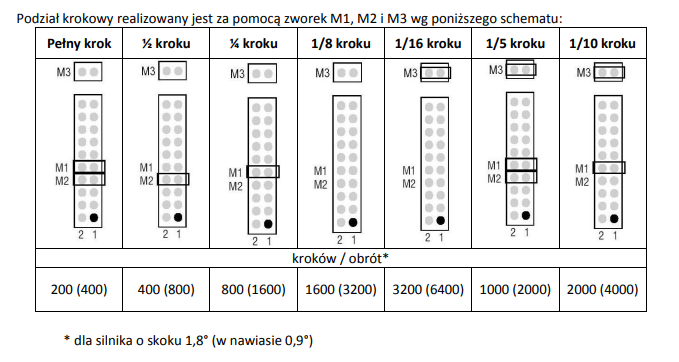
\includegraphics{pictures/stepy.png}}
    \caption{Tabelka z podziałami kroków drivera Wobit SMC64BP \cite{driver}}
    \label{stepy}
\end{figure}

%%%%%%%%%%%%%%%%%%%%%%%%%%%%%%%%%% SILNIK %%%%%%%%%%%%%%%%%%%%%%%%%%%%%%%%%%%%%%%

%%%%%%%%%%%%%%%%%%%%%%%%%%%%%%%%%% DRIVERY %%%%%%%%%%%%%%%%%%%%%%%%%%%%%%%%%%%%%%%
\section{Sterowniki silników krokowych} 

Do poruszania silnikami można użyć specjalizowanych układów wyposażonych we wzmacniacze mocy wraz z programowalnymi układami generującymi napięcia fazowe i ograniczającymi dopuszczalny prąd w uzwojeniach. Na rys. \ref{fig:driver} pokazano przykładowy cyfrowy interfejs sterujący \cite{driver2}. 

\begin{figure}[!htb]
    \centering
    \resizebox{13cm}{!}{
    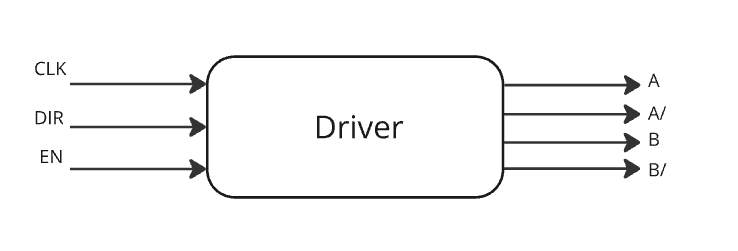
\includegraphics{pictures/driver.png}}
    \caption{Schemat blokowy sterownika}
    \label{fig:driver}
\end{figure}

\noindent Sygnał zezwolenia oznaczony jako \textbf{\textit{EN}} umożliwia działanie silnika pozwalając na przepływ prądu przez uzwojenia silnika. Wejście \textbf{\textit{DIR}} w zależności od swojego stanu określa kierunek obrotu silnika zgodnie lub przeciwnie do ruchu wskazówek zegara. Ostatnim z nich jest \textbf{\textit{CLK}}, który przyjmuje z urządzenia nadrzędnego sygnał PWM o danej częstotliwości definiując w ten sposób prędkość z jaką silnik ma się przemieszczać.\newline
\noindent Podczas realizacji pracy inżynierskiej użyte były dwa sterowniki silników oferowane przez firmę Wobit. Kontrolery SMC64 oraz SMC104 umożliwiają programowanie profili ruchu, określanie prędkości, przyspieszeń oraz docelowych pozycji dla każdego silnika. Dzięki temu SMC64 i SMC104 stanowią niezawodne i łatwe w utrzymaniu rozwiązania w środowiskach przemysłowych. Kontrolery mają możliwość obsługi różnych typów silników i oferują proste narzędzia do programowania, co sprawia, że są dosyć popularnym wyborem w aplikacjach wymagających dużej dokładności. Ich funkcje obejmują szeroki zakres zastosowań takich jak systemy CNC oraz systemy robotyki.

%%%%%%%%%%%%%%%%%%%%%%%%%%%%%%%%%% DRIVERY %%%%%%%%%%%%%%%%%%%%%%%%%%%%%%%%%%%%%%%

%%%%%%%%%%%%%%%%%%%%%%%%%%%%%%%%%% ENKODERY %%%%%%%%%%%%%%%%%%%%%%%%%%%%%%%%%%%%%%%
\section{Enkodery}
Enkodery to urządzenia służące do precyzyjnych pomiarów pozycji, kierunku ruchu wału lub innego obracającego się elementu. W zależności od metody wykonywania pomiarów, enkodery można podzielić na dwa główne rodzaje - enkodery optyczne inkrementalne i absolutne \cite{enkoder}.\newline 

\noindent Ze względu na swoją prostotę prawdopodobnie najczęściej spotykanym typem są enkodery inkrementalne. Ich działanie polega na generowaniu impulsów podczas obrotu obiektów. Enkoder inkrementalny składa się zazwyczaj z tarczy, na której znajdują się równomiernie rozmieszczone szczeliny lub ciemne i jasne segmenty, które przepuszczają lub blokują światło emitowane przez diodę LED. Światło pada na czujnik zliczający przejścia, generując w ten sposób impulsy. Każdy impuls odpowiada określonemu przemieszczeniu wału, co umożliwia obliczenie kąta obrotu oraz prędkości. Kolejnym istotnym elementem enkoderów inkrementalnych jest kanał referencyjny (kanał Z), który generuje impuls zerowy przy każdym pełnym obrocie wału. Ten pojedynczy impuls może być używany do ustalenia pozycji referencyjnej, co pozwala na wyzerowanie licznika i rozpoczęcie zliczania od tego punktu. Standardowe enkodery inkrementalne składają się z dwóch kanałów sygnałów (A i B), które są przesunięte względem siebie o 90 stopni (tzw. sygnały kwadraturowe). Dzięki temu możliwe jest określenie kierunku obrotu wału poprzez porównanie sygnałów A i B pozwalające ustalić, czy np. wał obraca się zgodnie z ruchem wskazówek zegara.\newline 
\noindent Enkodery absolutne różnią się od enkoderów inkrementalnych w sposobie definiowania pozycji wału, ponieważ każda pozycja takiego wału jest kodowana w sposób unikatowy. Dlatego, nawet jeśli zasilanie zostanie wyłączone, enkoder absolutny pamięta aktualną pozycję wału. Enkodery absolutne to enkodery z tarczą kodową, na której każda pozycja jest oznaczona charakterystycznym wzorem, który może być odczytywany przez różne czujniki. W zależności od zastosowanego kodu rozdzielczość enkodera absolutnego wynika z przyjętej reprezentacji kąta i liczby detektorów, umożliwiając precyzyjne określenie pozycji z dokładnością do ułamków stopnia. Sygnał wyjściowy jest reprezentowany przez liczby binarne lub inny kod cyfrowy, który definiuje konkretną pozycję. Taki kod może być kodem Gray’a, który minimalizuje błędy odczytu przy przełączaniu pomiędzy sąsiadującymi pozycjami. Z tego powodu enkodery absolutne są mniej podatne na zakłócenia i błędy w odczycie pozycji.\newline 
\noindent Ważnym aspektem w przypadku enkoderów jest pojęcie pozycji referencyjnej ustawionej ręcznie lub przez system sterujący. W inkrementalnym zwykle odbywa się to przez odnalezienie impulsu referencyjnego (kanał Z) generowanego raz na obrót. Po osiągnięciu tej pozycji system sterujący może zresetować licznik impulsów i rozpocząć zliczanie od zera. W enkoderach absolutnych nie ma potrzeby ustawiania pozycji referencyjnej, ponieważ każda pozycja jest odczytywana bezpośrednio jako unikatowa wartość eliminując potrzebę resetowania licznika.

\begin{figure}[!htb]
    \centering
    \resizebox{14cm}{!}{
    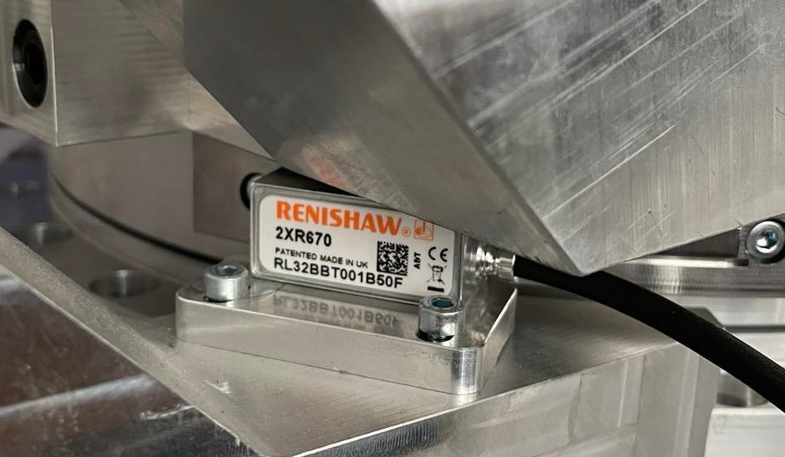
\includegraphics{pictures/enkoder.png}}
    \label{enkoder}
    \caption{Model zamontowanego enkodera na stanowisku}
\end{figure}

%%%%%%%%%%%%%%%%%%%%%%%%%%%%%%%%%% ENKODERY %%%%%%%%%%%%%%%%%%%%%%%%%%%%%%%%%%%%%%%

%%%%%%%%%%%%%%%%%%%%%%%%%%%%%%%%%% MIKROKONTROLER %%%%%%%%%%%%%%%%%%%%%%%%%%%%%%%%%%%%%%%
\section{Mikrokontroler}
Podstawowym elementem układu sterowania uchwytem odpowiedzialnym za odczyt z pozycji, obsługę sterowników silników, realizacji algorytmu sterowania pozycyjnego potrzebne było urządzenie wielofunkcyjne. Z ogólno dostępnych i tanich rozwiązań zdecydowaliśmy się na minikomputer, a dokładniej model płytki programistycznej STM32H743ZI z zaawansowaną platformą deweloperską opartą na mikrokontrolerze z serii STM32H7 zaprojektowaną przez firmę STMicroelectronics. Miktrokontrolery te charakteryzują się dużą wydajnością, wysoką częstotliwością taktowania oraz rozbudowanymi możliwościami komunikacyjnymi, co sprawia, że są idealnym rozwiązaniem do zastosowań wymagających dużej mocy obliczeniowej oraz wszechstronnej komunikacji. Wspomniany rodzaj płytki programowalnej STM32 Nucleo-144 oferuje bardzo wysoką wydajność obliczeniową dzięki rdzeniowi ARM Cortex-M7 działającemu z częstotliwością nawet do 480 MHz. Zawiera również bogaty zestaw peryferiów i dużą ilość pamięci (do 2 MB Flash oraz 1 MB RAM). Ponadto, STM32H743ZI oferuje szereg funkcji, które znacząco ułatwiają proces projektowania oraz integracji aplikacji takich jak zintegrowany debugger/programmer ST-LINK eliminując potrzebę stosowania zewnętrznych narzędzi do debugowania i programowania. Jest to duże udogodnienie przyspieszające proces rozwoju i testowania aplikacji. \newline 
\noindent Płytka STM32 Nucleo-144 oferuje też pełną kompatybilność z popularnym standardem ARDUINO® Uno V3 pozwalając na łatwą integrację z szeroką gamą dostępnych rozszerzeń odnoszących sie do płytek nasadkowych tzw. shields. Dodatkowo, złącza ST morpho oraz Zio zapewniają jeszcze większe możliwości rozbudowy płytki o dodatkowe moduły i peryferia. Z kolei, dzięki złączu MIPI20 można podłączyć moduły kamer, co może być istotnym elementem w projektach związanych z przetwarzaniem obrazu lub monitorowaniem wideo. \newline 
\noindent Wspomniany model udostępnia interfejsy komunikacyjne, w tym Ethernet (RJ45), USB w wersjach pełnej prędkości oraz USB OTG pozwalając na łatwą komunikację z innymi urządzeniami. Jednocześnie zawiera również interfejsy komunikacyjne takie jak I2C lub SPI zdatnych do pobierania informacji z urządzeń takich jak chociażby enkodery. \newline
\noindent Warto także nadmienić, że mikronkontroler wspiera bogaty ekosystem oprogramowania STM32Cube, który obejmuje biblioteki, przykłady kodu oraz narzędzia do konfiguracji peryferiów. Dodatkowo, płytka wspiera popularne systemy operacyjne czasu rzeczywistego FreeRTOS, co jest przydatne w bardziej zaawansowanych aplikacjach wspomagających między innymi pracę serwera sieciowego.

%%%%%%%%%%%%%%%%%%%%%%%%%%%%%%%%%% MIKROKONTROLER %%%%%%%%%%%%%%%%%%%%%%%%%%%%%%%%%%%%%%%

%%%%%%%%%%%%%%%%%%%%%%%%%%%%%%%%%% SWITCH/HUB %%%%%%%%%%%%%%%%%%%%%%%%%%%%%%%%%%%%%%%
\section{Switch/Hub}
Switch i Hub stanowią urządzenia sieciowe służące do łączenia komputerów i innych urządzeń w sieciach lokalnych nazywanych. Pomimo podobnej funkcji oraz wzajemnego wpływu na efektywność i wydajność sieci różnią się sposobem działania. \cite{net}.\newline
\noindent Huby to prostsze i z reguły tanie sprzęty sieciowe, które działają jako punkt rozdzielający sygnał sieciowy. Wszystkie urządzenia podłączone do hub-a są ze sobą połączone w sposób równoległy. Kiedy transmitter wysyła dane hub przekazuje ten sygnał do wszystkich portów. Nie analizuje adresów docelowych, dlatego każde urządzenie w sieci otrzymuje dane, nawet jeśli nie są one do niego skierowane. Receivery są więc zmuszone zignorować dostaroczne do nich pakiety informacji. \newline
\noindent W przeciwieństwie do hubów switche to bardziej zaawansowane urządzenie sieciowe, które działają na wyższej w warstwie łącza danych modelu OSI, czyli na warstwie drugiej. Analizują adresy MAC urządzeń podłączonych w jego porty i definiują wewnętrzną tablicę MAC, według której następuje przesył pakietów. Gdy dane docierają do switch-a sprawdza on adres MAC docelowy wysyłając dane bezpośrednio do odpowiedniego portu, zamiast rozsyłać je do wszystkich urządzeń. Dzięki temu switch minimalizuje ruch w sieci i zwiększa wydajność, ponieważ tylko właściwe urządzenie odbiera dane. \newline
\noindent W naszej aplikacji jedynym urządzeniem odbierającym dane z serwera jest mikrokontroler. Aspekt wydajności nie był najważniejszy, dzięki czemu można było wybrać podstawową opcję, czyli hub. 

%%%%%%%%%%%%%%%%%%%%%%%%%%%%%%%%%% SWITCH/HUB %%%%%%%%%%%%%%%%%%%%%%%%%%%%%%%%%%%%%%%
\newpage 